\documentclass{llncs}

\usepackage{booktabs}
\usepackage[ruled]{algorithm2e} % For algorithms

\usepackage{siunitx}
\usepackage{graphicx}
\usepackage{multirow}
\usepackage[caption=false]{subfig}
\usepackage[capitalise]{cleveref}
\usepackage{todonotes}

\begin{document}

\title{Audio Interface of an Active Perception Navigation Aid for People with Visual Impairments}
\titlerunning{Active Perception Interface for People with Visual Impairments}

\author{Jacobus C. Lock\inst{1} \and 
Iain Gilchrist\inst{2} \and
Grzegorz Cielniak\inst{1} \and
Nicola Bellotto\inst{1}}

\institute{University of Lincoln \email{\{jlock, gcielniak, nbellotto\}@lincoln.ac.uk} \url{https://lcas.github.io/ActiVis/} \and
	   University of Bristol \email{i.d.gilchrist@bristol.ac.uk}}

\authorrunning{Jacobus C. Lock et.\ al.}

\maketitle

\begin{abstract}
	%Our aim is to build a portable active navigation system for people with visual impairments that uses active perception techniques and a combination of feedback modes to identify a scene and guide a user to their destination.
	%Such a system requires a non-visual feedback interface and in this paper we investigate the effectiveness of a spatial audio tone with a varying pitch component, played through bone-conducting headphones, in conveying the pan and tilt angles of a target to the user in a pointing task.
	%The secondary goal is to determine how variations to the pitch's rate of change affect the user's performance.
	%For this, we conducted a set of experiments with both blindfolded participants and participants with visual impairments and found that, with some limitations, a spatialised audio tone with a varying pitch component can successfully convey a target's pan and tilt angles. 
\keywords{Human-machine interface \and vision impairment \and spatialised sound \and varying pitch, pointing task}
\end{abstract} 

\section{Introduction}

In recent years, governments have spearheaded numerous initiatives to support people with disabilities and enable them to play a more active role in modern society.
The UK's Royal National Institute of Blind People (RNIB) for example has prioritised improving access to everyday services and products, such as public transport and mobile apps~\cite{rnib-objectives}.
Improvements in modern computing have made it possible for new and innovative solutions to these problems to come to the fore.
In particular, researchers in the active vision field have have made much progress in enabling machines to autonomously manipulate cameras to gather information about an environment for mapping and object and object finding tasks~\cite{bajcsy2018revisiting}.
There is, however, a significant research question about whether techniques from active machine vision can be applied to humans, i.e.\ can a machine identify a point of interest in a scene and direct a human, instead of an electronic servo, to focus on that point?
If this can be done, it would be beneficial to people with visual impairments and will augment their ability to search for an arbitrary point or object of interest and identify an unknown scene. 

The ActiVis project aims to deliver a mobile guidance system based on the Google Project Tango platform\footnote{\url{https://en.wikipedia.org/wiki/Tango\_(platform)}}, pictured in \cref{fig:tango-headphone}, that will ultimately be able to guide a user with vision impairments on the last leg of their journey, i.e.\ the so-called `last 10-yard problem'. 
The entire platform is based on a Google Project Tango device that provides access to powerful real-time localisation (through IMU measurements and landmark tracking) and image-processing facilities and provides access to Android's full range of interface tools and IO options. 
Furthermore, a set of bone-conducting headphones (pictured in \cref{fig:tango-headphone}) that are placed on a user's cheekbones instead of their ears and do not interfere with normal hearing, are used to transmit the audio signals to the user.
The system will provide real-time guidance instructions for the user to follow and it is important that these instructions are easily understood and are not perceived as a cognitive burden. 
Humans are naturally able to determine the 3D position of a sound source and by exploiting this ability, the system's guidance instructions can naturally be interpreted without posing a unnecessary burdensome cognitive load.
A sound source can be spatialised by adjusting a tone's spectral make-up (elevation angle), time delay and level difference (pan angle) and the intensity (distance).
Here only the pan and elevation positions are transmitted.
However, since bone-conducting headphones bypass the outer ear structure, their spectral signature cannot properly be interpreted and we therefore convey the target's elevation angle by simply adjusting the tone's pitch.

%For this work, we investigate implementing such an interface that uses audio signals to transmit guidance instructions by exploiting the human auditory and psychoacoustic systems. 
%Initially the interface is implemented in 2D only (pan and tilt dimensions) to provide the user with audio instructions on where to point the device and our approach was validated through a set of simple pointing tasks. 

\begin{figure}
  \centering
  %\subfloat[]{\label{fig:tango-headphone}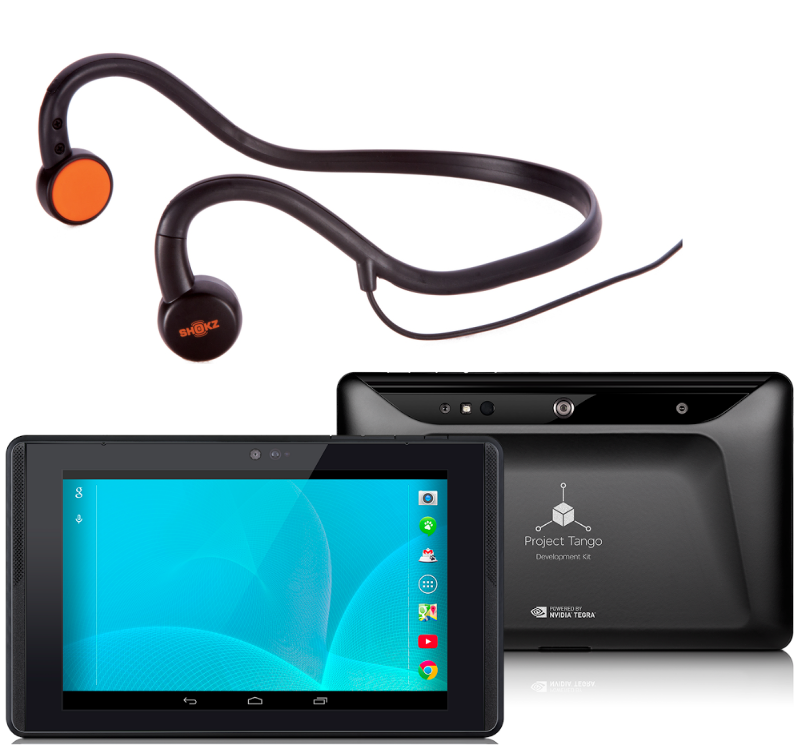
\includegraphics[width=0.5\columnwidth]{figures/tango_headphone.png}}
  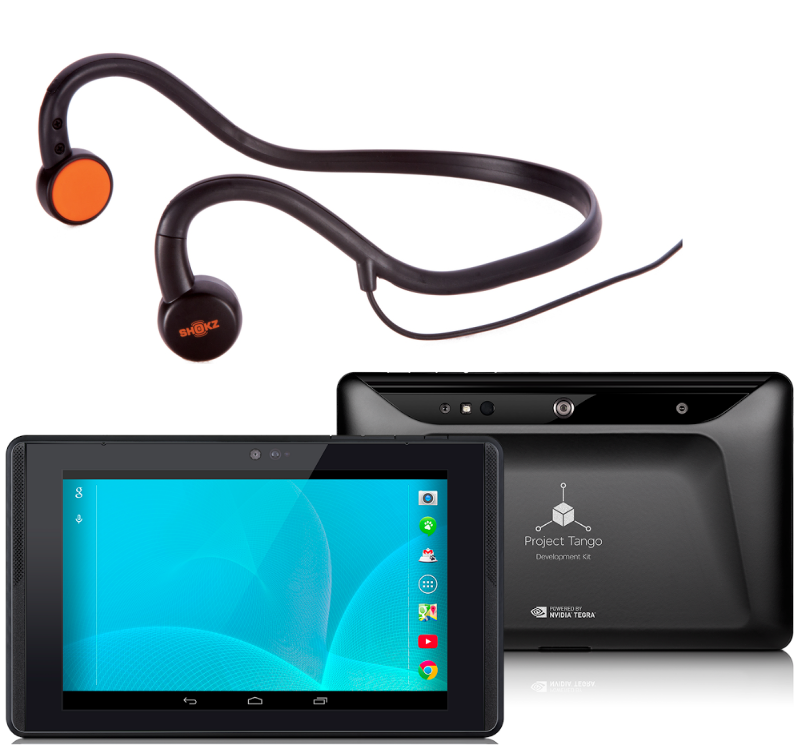
\includegraphics[width=0.5\columnwidth]{figures/tango_headphone.png}}
  %~
  %\subfloat[]{\label{fig:participant}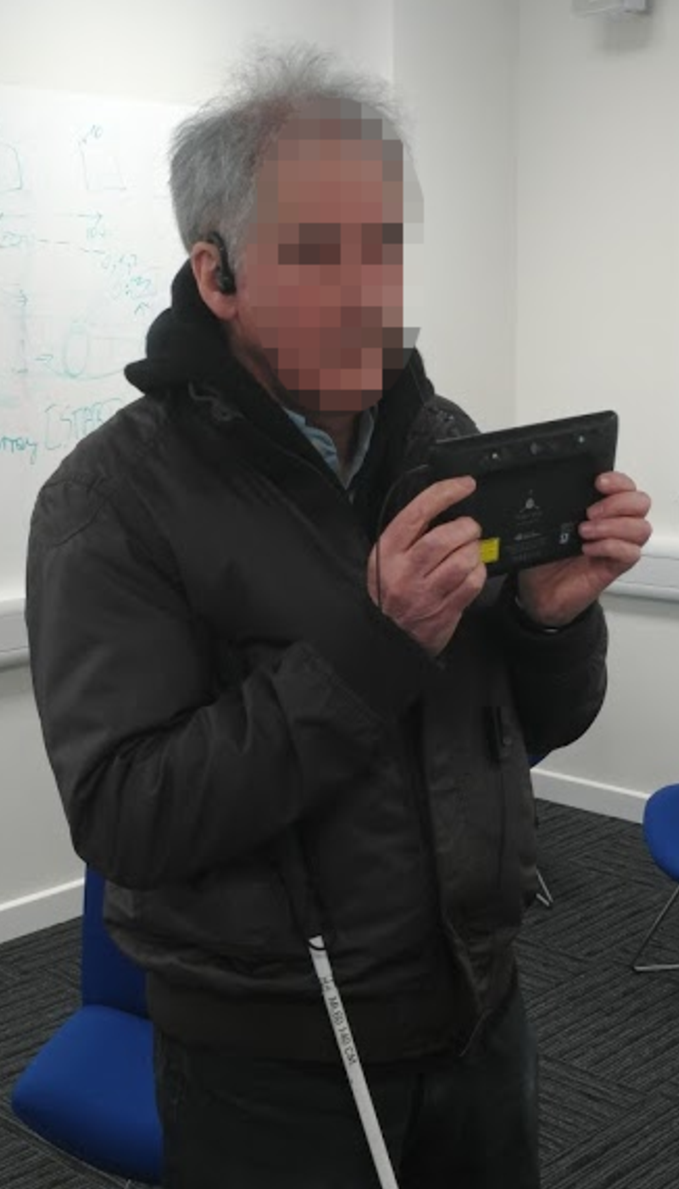
\includegraphics[width=0.35\columnwidth]{figures/vi_participant.pdf}}
  \caption{Pictures of the Tango device and bone-conducting headphones the system is based on (left) and both in use in an experiment (right).}\label{fig:tango-headphone}
\end{figure}

A similar approach was used in \todo{ref previous varying pitch study}, but the study did not focus on the interface's efficacy.
Indeed, this work serves as an initial study into such an interface.
The contribution of this work is an effective approach to addressing the shortcomings of bone-conducting headphones in transmitting spatialised sounds through a generic sound library, as well as initial experiments demonstrating its effectiveness.

The rest of the paper is \todo{lay out rest of paper}

\section{Previous Work}

Work on guiding/directing people (vibration, audio, voice)
Show preference studies

Guidance instruction delivery modes using haptic, audio and vocal feedback for non-visual human-machine-interfaces (HMI) have been investigated before. 

Previous work on HRTF stuff

\section{Interface Implementation}

\subsection{Human Audio Localisation}

Humans localise a sound source in 3 dimensions by considering cues recorded in one ear (monaural cues) and comparing cues derived at both ears (binaural cues).
The binaural cues include time differences of arrival and intensity differences that help to determine a source's location on the horizontal plane.
Monaural cues are taken from the interaction of the sound with the human anatomy, e.g.\ head, shoulders, outer ear, before it enters the ear canal.
The user's anatomy acts as a filter and the direction the sound wave hits the body activates different filter resonances, attenuating or accentuating different frequency bands.
When the modified sound enters the inner ear, the human brain is able to analyse the frequency response and accurately determine the position of the sound source on the vertical plane. 
The distance to the source is simply derived as the intensity, or volume, of the source, i.e.\ a louder sound would appear closer to the user than a softer one does. 

When an audio signal is transmitted via a set of speakers or headsets, it can be transformed to mimic the characteristics of a natural sound sources before it is transmitted, thereby tricking the brain into believing a sound is located at some arbitrary position.
Such a transformation can be done using a head-related transfer function (HRTF) and a pair of stereo headsets or speakers.
An HRTF is a mathematical function that simulates the response signal of a human head and is derived by capturing key characteristics that affect the monaural and binaural responses, such as the user's hearing levels and head size, etc.
Since hearing responses can be quite unique between user's, the best results would be observed if each user had their own customised HRTF.\
Given the complicated process involved to capture the required user characteristics, making unique HRTFs is often an untenable solution and using average values (e.g.\ head measurements, height, etc.) have shown to produce acceptable results.\todo{cite HRTF papers}

\subsection{Interface Design}

The guidance target is presented to the user in terms of pan and elevation angles, indicating the angle adjustments that are required to point the device camera at the target location.
Spatialised audio signals are well-suited to the task, displaying similar levels of performance to vocal feedback, but with less cognitive load and higher resolution.
However, the audio guidance signals are delivered to the user with a set of bone-conducting headphones that bypass the user's outer-ear structure and since this structure plays an important role in localising a sound source's elevation, an alternative mode of conveying the elevation angle is required.
For this work, we propose a simple linear adjustment to the signal's pitch as a function of the elevation angle. 

\subsubsection{Pan}

Binaural comparison cues are used to 

\subsubsection{Elevation}

\subsection{Implementation}

\section{Experiment and Results}

\subsection{Apparatus}

\subsection{Procedure}

\subsection{Results}

\section{Conclusion}

%\section{Previous Work}\label{sec:lit-review}

%Earlier attempts at improving a person with visual impairment's navigation experience involved outfitting the commonly-used walking cane with remote detection systems, such as sonar, radar and RFID tags, to transform a cane into an early-warning system~\cite{ulrich1997,marion2008batcane,faria2010electronic,willis2005}.
%Bluetooth tags and a smartphone can be used in a similar manner~\cite{sato2017navcog3}.
%However, the expense and effort of maintaining such tags make them less attractive for wide-scale adoption.
%Computer vision-based systems provide a good compromise between usability, cost and accuracy.
%One solution is to use RGB-D depth sensing cameras, which are becoming increasingly accurate and cost-effective, to build a 3D image map of the environment, and guiding a user through it~\cite{lee2015,rodriguez2012obstacle}.
%Alternatively, object recognition techniques can be used to detect various objects and landmarks, such as doors, staircases, etc., and communicate their relative location to the user~\cite{schauerte2012assistive,tian2013b,fiannaca2014headlock}, or use audio instructions to guide a user to fully capture an object of interest~\cite{vazquez2012helping}. 

%An important feature of user-centric systems is a human-machine interface (HMI) that enables effective two-way communication between the system and the user.
%Surveys found that people with visual impairments prefer receiving instructions in the form of speech and haptic feedback cues~\cite{khoo2016multimodal,ross2000wearable,vazquez2012helping}.
%However, haptic feedback modes typically have a lower bandwidth when compared to audio feedback and also require the user to wear a special device in order to transmit the signals effectively.
%Work has also been done in translating a visual scene into non-visual formats, with so-called sensory substitution systems (e.g. `The Voice'~\cite{meijer2010}) and virtual audio reality (VAR) systems~\cite{frauenberger2003} reporting favourable results.
%However, The Voice has a very steep learning curve that has proven to be a significant barrier to entry and with VAR systems, it is not clear how unknown environments, where markers have not yet been encoded, would be handled and described to the user. 

%Previous experiments have determined that people are able to find the location of a stationary sound source with an error of $\pm$\SI{35}{\degree}, in both the pan and tilt dimensions~\cite{zwiers2001spatial}, for both early-blind and normally-sighted people.
%However, in~\cite{lewald2013exceptional,lessard1998early} it was found that the blind have a clear advantage in localisation accuracy over sighted people when presented with more complex tasks, such as targets in motion and narrow-band stimuli, with~\cite{lewald2013exceptional} reporting an average absolute localisation error of around \SI{10}{\degree} in the pan and tilt dimensions.
%Researchers have used simulated spatialised audio to inform the user of the sound source's direction~\cite{holland2002audiogps,kammoun2012navigation,rebillat2009smart,menelas2010audio,wilson2007swan,zotkin2004rendering}.
%In these works, a sound was played through a set of headphones and the source spatialised with a head-related transfer function (HRTF), tricking the listener into thinking the sound source was located at some arbitrary 3D location.
%There are also experimental results about how well users can find targets presented with spatial sound in the tilt and panning dimensions with normal headphones~\cite{katz2011spatial,zwiers2001spatial}, as well as work that has shown similar levels of localisation performance between normal and bone-conducting headphones in the pan dimension~\cite{macdonald2006spatial}.
%However, to our knowledge no extensive work or experiments have been done to determine how well users respond to tilt adjustment instructions using a tone with \textit{varying pitch}, in particular when using bone-conducting headphones, and how changes to this tone's behaviour affects performance. 

%\section{Portable Navigation System}\label{sec:portable-navigation}

%\subsection{System Setup}

%Our ultimate goal is to deliver a navigation system that can guide a user with visual impairments on the last leg of their journey (e.g.\ to a specific aisle and shelf in a shop) using only a mobile phone.
%A large amount of data need to be translated from a visual form into a format that is useful to people with limited or no vision.
%We therefore plan to use a combination of voice, audio and vibration cues to translate visual navigation data as effectively as possible and overcome the bandwidth limitation of the human ear. 
%However, for this paper, we only considered the spatialised audio mode and its variation in pitch in order to determine its effectiveness in conveying a target's pan and tilt angles.

%The system is based on a concept proposed in~\cite{bellotto2013,lock2017portable}, which uses a Google Tango device.
%The navigation system is based on a Google Tango tablet, an Android-based device that comes equipped with an RGB-D camera to sense colour and depth and combines an inertial measurement unit (IMU) with powerful and robust landmark recognition and image processing algorithms to localise itself in real-time.
%An added benefit of this platform is its familiar, compact form-factor which will help overcome the hurdle of user-acceptance and usability.
%The guidance instructions are presented through a set of bone-conducting headphones (see \cref{fig:tango-headphone}) that are placed externally on a user's head so that the system does not occlude the perception of real-world sounds and does not interfere with a user's normal hearing function.

%A diagram of the experimental system pipeline is shown in \cref{fig:pipeline}, where the arrows indicate the direction of the flow of information.
%When the user taps the Tango's screen, a new virtual target is generated and its coordinates are sent to the audio generation module, along with the device's current position and orientation.
%The audio generator then produces a tone based on the difference between the device and target's positions and sends it to the audio output channel, which plays it back to the user.
%The WiFi recording module is constantly monitoring the different parameter values of the device and target's positions, as well as the system's output, and records it to a remotely stored datafile. 

%\begin{figure}
  %\centering
  %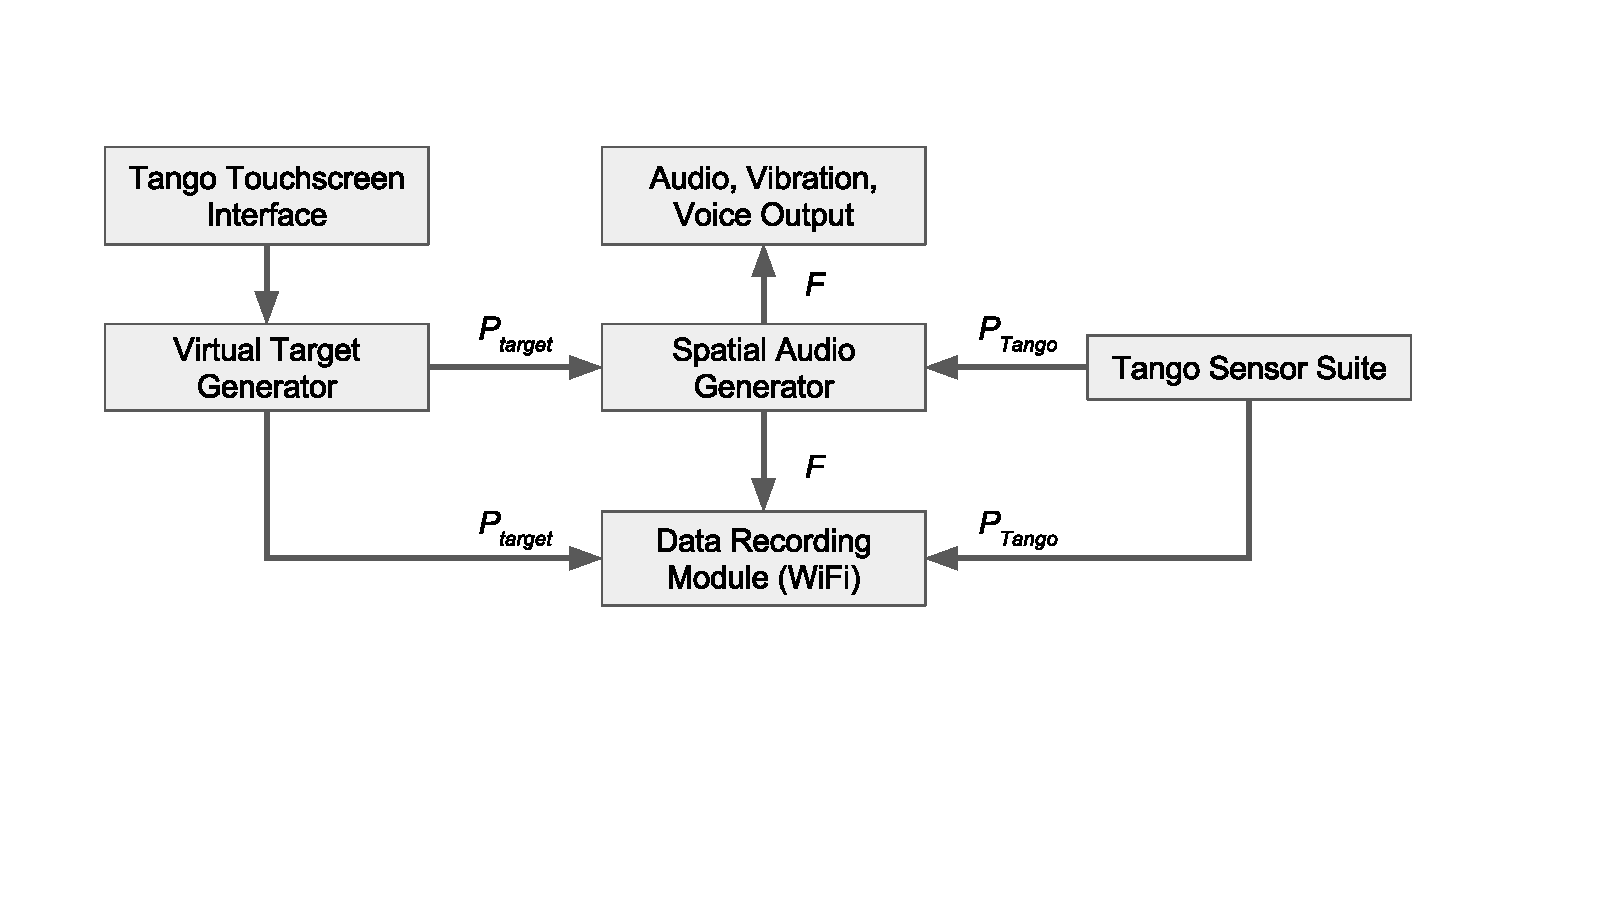
\includegraphics[clip=true, trim=0 120 80 50, width=1.0\columnwidth]{figures/pipeline.pdf}
  %\caption{A diagram of the individual system components and their communication pipelines. $F$ indicates a feedback signal and $P$ a pose signal. }\label{fig:pipeline}
%\end{figure}

%\subsection{Audio Interface}

%The audio component is responsible for conveying the 2D position of a target on the vertical plane, shown by \cref{fig:cam-coords}, in terms of pan and tilt angles.
%The audio signal is a continuous \SI{10}{\hertz} sinusoidal sound wave that is played to the user through bone-conducting headphones.
%We use a sinusoidal wave here because it is relatively simple to manipulate and analyse and will be replaced by a richer, more natural tone at a later stage. 

%The audio is spatialised in the pan dimension using the OpenAL\footnote{\url{http://openal.org}} sound library's HRTF, while the tilt angle is conveyed by varying the audio tone's pitch.
%We use this approach because the external set of bone-conducting headphones plays the sound through a user's cheekbones instead of their outer ears, bypassing the ears' pennae that provide the ability to localise elevated sound sources~\cite{roffler1968factors,algazi2001elevation}.
%This makes an HRTF less effective in conveying the target's elevation and therefore needs to be conveyed using another method; by varying the tone's pitch in this case.
%The difference between the target's angular position and the device's angular orientation are used to generate the audio signals. 

%\subsubsection{Pan Direction}

%The pan angle ($\phi$) describes the angle which the user needs to rotate the camera vector, $C$, around the $z$-axis shown in \cref{fig:cam-coords}, i.e.\ how far the target is to the left or right of the user.
%We use an HRTF to add a spatial element to the audio tone that is played to the user, placing the sound source at the target's location. 
%Humans determine a sound source's pan direction by subconsciously analysing the inter-aural time difference (IID) between a sound reaching both of your ears: the greater the IID, the greater the perceived angular distance to the sound source~\cite{wightman1992dominant}.

%We implement OpenAL's default HRTF, based on the MIT's KEMAR dataset\footnote{\url{http://sound.media.mit.edu/resources/KEMAR.html}}, to generate a sinusoidal sound wave based on the difference between the user and target's positions.
%The library takes position values as input and outputs a tone based on the angle between the two position vectors. 

%\subsubsection{Tilt Direction}

%The system adjusts the tone's pitch ($f$) to convey the target's tilt angle ($\theta$) w.r.t.\ $C$. 
%Here, a high pitch means the target is above $C$ (i.e.\ the user should look up) and a low pitch means the target is below $C$ (the user should look down).
%This high/low association scheme is chosen because humans naturally associate high-pitched sounds with higher objects and lower-pitched noises with lower objects~\cite{pratt1930spatial,blauert1997spatial}.
%We use a logarithmic, octave-based gain function for the pitch, since an increase in octave provides a distinct perceptible change while keeping the timbre roughly constant~\cite{shepard1964circularity}.

%We wish to determine how the gradient, $m$, of the pitch gain as a function of $\theta$ (i.e.\ $m = \frac{df}{d\theta}$) affects a user's performance, e.g.\ does a greater $m$ lead to an increased target acquisition rate?
%For this we select 3 different pitch settings, referred to henceforth as $m_l$, $m_m$ and $m_h$ for the smallest, middle and highest gain gradients respectively. 
%To find these gradients, we set the maximum and minimum limits for $\theta$ and the maximum and minimum frequencies for $f$ for each respective setting.
%Furthermore, for the sake of consistency and between the different settings, each gradient generates the same pitch when $C$ is level with the target's tilt. 

%After practical tests with the device and headphones, we set the neutral, on-target tone to $f_{512} =$ \SI{512}{\hertz} for its audibility.
%For $m_l$, we set $f_{max}$ and $f_{min}$ to 1 octave higher and lower than $f_{512}$, giving limits of \SI{1024}{\hertz} and \SI{256}{\hertz} respectively.
%For $m_m$, the $f_{max}$ and $f_{min}$ are set to 2 octaves higher and lower than $f_{512}$ (\SI{2048}{\hertz} and \SI{128}{\hertz}) and $m_h$ to 3 octaves higher and lower (\SI{4096}{\hertz} and \SI{64}{\hertz}).
%These limits were selected for practical reasons, because the bone conducting headphones have low volume gain at the frequency spectrum extremes, making it difficult to hear. 
%The values of $m_l, m_m, m_h$ are visualised in \cref{fig:pitch-gain}.

%\begin{figure}
  %\centering
  %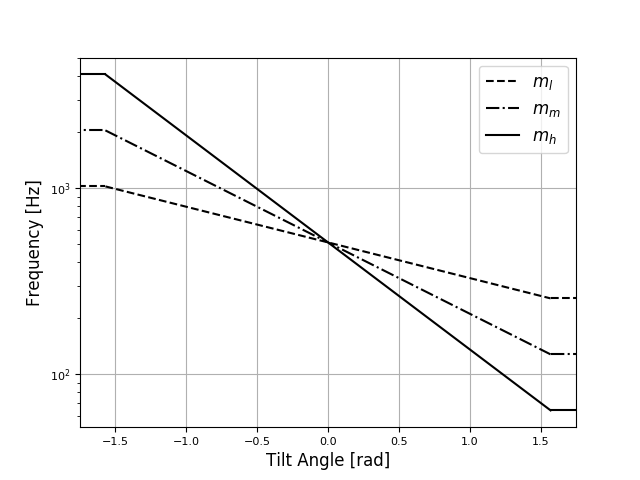
\includegraphics[clip, trim=0 0 0 40, width=1.0\columnwidth]{figures/pitch_gain_functions.png}
  %\caption{The pitch gain functions for the 3 different gain settings ($y$-axis in log scale). }\label{fig:pitch-gain}
%\end{figure}

%We set the range of angles the system can convey to $[-\frac{\pi}{2}; \frac{\pi}{2}]$; anything outside this range implies that the target is behind the user and was not considered in this series of experiments. 
%The \SI{0}{\radian} position is directly in front of the user.
%With these limits, $f$ can be determined with 

%\begin{equation}\label{eq:frequency}
  %f(\theta) = 2^{b\theta + c},
%\end{equation}
%where $b$ and $c$ for each setting can be calculated according to the given setting's pitch and angle limits.% and a linear graph equation (i.e.\ $f - f_1 = b(\theta - \theta_1), b=\frac{\Delta f}{\Delta\theta}$).

%\section{Target Search Experiment}\label{sec:experiments}

%We conducted a set of experiments to evaluate the audio interface's effectiveness at driving a user to point the camera at a target in the pan and tilt dimensions.
%Furthermore, we wish to see how changes to $m$ affect a user's performance.

%We recruited 2 groups of participants for the experiments.
%Group $G1$ consists of 42 young adults (mostly students) with healthy eyesight, with 10 males and 32 females being $20\pm1.5$ years old on average.
%This group was blindfolded throughout the experiment and forms the bulk of the participant population.
%Group $G2$ is made up of 3 legally blind adults with little to no light perception (3 males, average age of $40\pm8$ years). 
%This group makes up less than 10\% of the total experiment population, but provided valuable subjective feedback that will help improve the system before evaluating it with a larger group of people with vision impairments. 
%All participants joined the experiment on a voluntary basis with written consent and have no other impairments that affected their interpretation of the audio guidance cues.

%For the experiment, the participants were given a Tango tablet device, running an app written for this experiment, and a pair of AfterShockz Sportz3' bone conducting headphones (both pictured in use in \cref{fig:participant}) and were blindfolded where appropriate.
%The app generates a virtual target, one at a time at a constant \SI{2}{\metre} from the participant, and uses the device's pose measurements to determine $\phi$ and $\theta$.
%These angles are then used to generate and present the user with the audio signal to direct them to the target. 
%As the participant rotates the camera, $\phi$ and $\theta$ are adjusted and the audio signal changes to reflect these changes.
%When a participant believes that they are pointing at the target, they tap the screen which generates a new target target which they are then directed to. 
%Each participant was given 28 targets in total that were randomly generated and equally spread across 4 quadrants to avoid clustering. 
%After the 28 targets were found, $m$ was adjusted and the experiment was repeated. 
%The order in which the gradient setting was changed for each participant was randomised to minimise the learning effect.
%The app streams various data on the current device and target poses to a laptop computer via a WiFi connection in real-time. 
%Before the experiment session started, each participant was given some time to familiarise themselves with the device and was given the opportunity to learn what the $f_{512}$ `on-target' and on-centre tone sounds like that will mean that they are pointing at the target.

%The measure of performance here is the accuracy with which a user points the camera towards a target.
%The accuracy is taken as the angular difference between $C$ and the target's position at the time the participant tapped the screen.
%A smaller error indicates more accurate results.
%The pan and tilt results are separated to understand the effect of changing the gradient setting has on either dimension's accuracy.
%To minimise the speed/accuracy biases in the results, we asked the participants to focus on finding the targets as well as they could without worrying about the time it took.  

%\section{Results and Discussion}\label{sec:results}

%The results for the participants are given by the 2D histograms in \cref{fig:err-results}, where the pan error is on the abscissa and the tilt error on the ordinates.
%A set of box-plots of the angular errors' median and standard deviations are given in \cref{fig:err-boxplot} for the $m_l, m_m$ and $m_h$ settings. 
%The results for $G1$ are summarised in \cref{tab:results}, while the results for $G2$ are given in \cref{tab:vi-results}.

%\begin{figure}
  %\centering
  %\subfloat[Results for the $m_l$ setting.]{\label{fig:err-results-lo}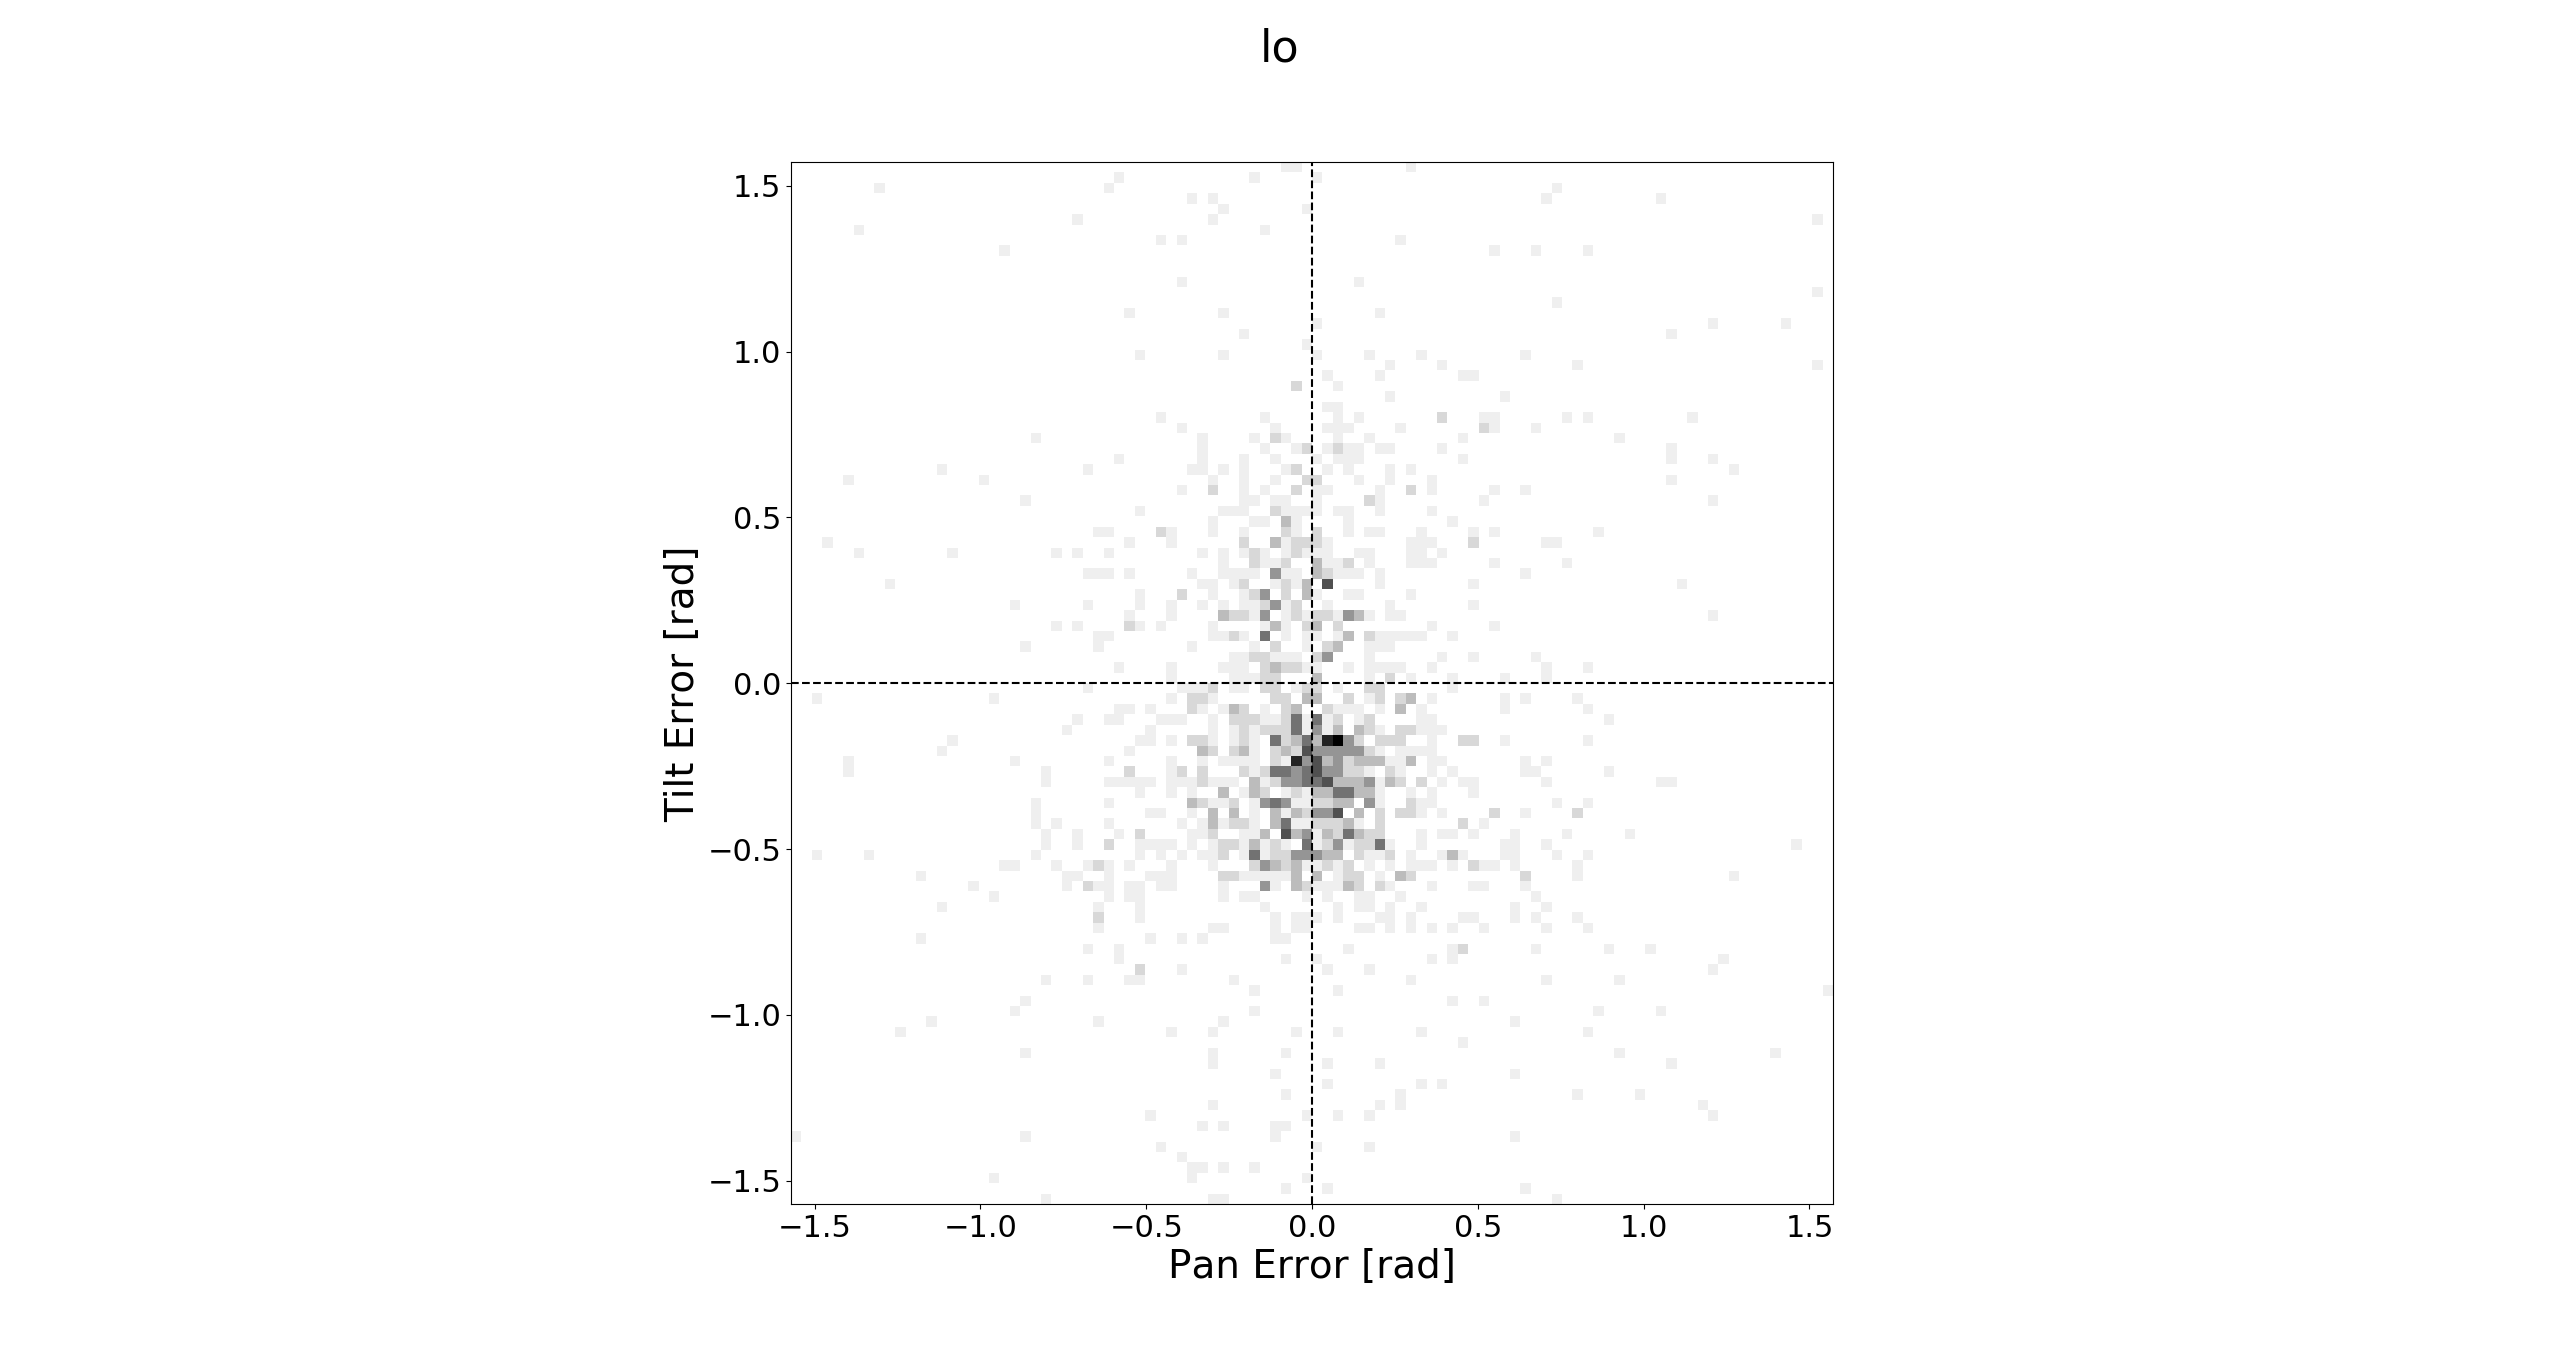
\includegraphics[clip, trim=450 0 450 110, width=0.8\columnwidth]{figures/err_lo.png}}

  %\subfloat[Results for the $m_m$ setting.]{\label{fig:err-results-med}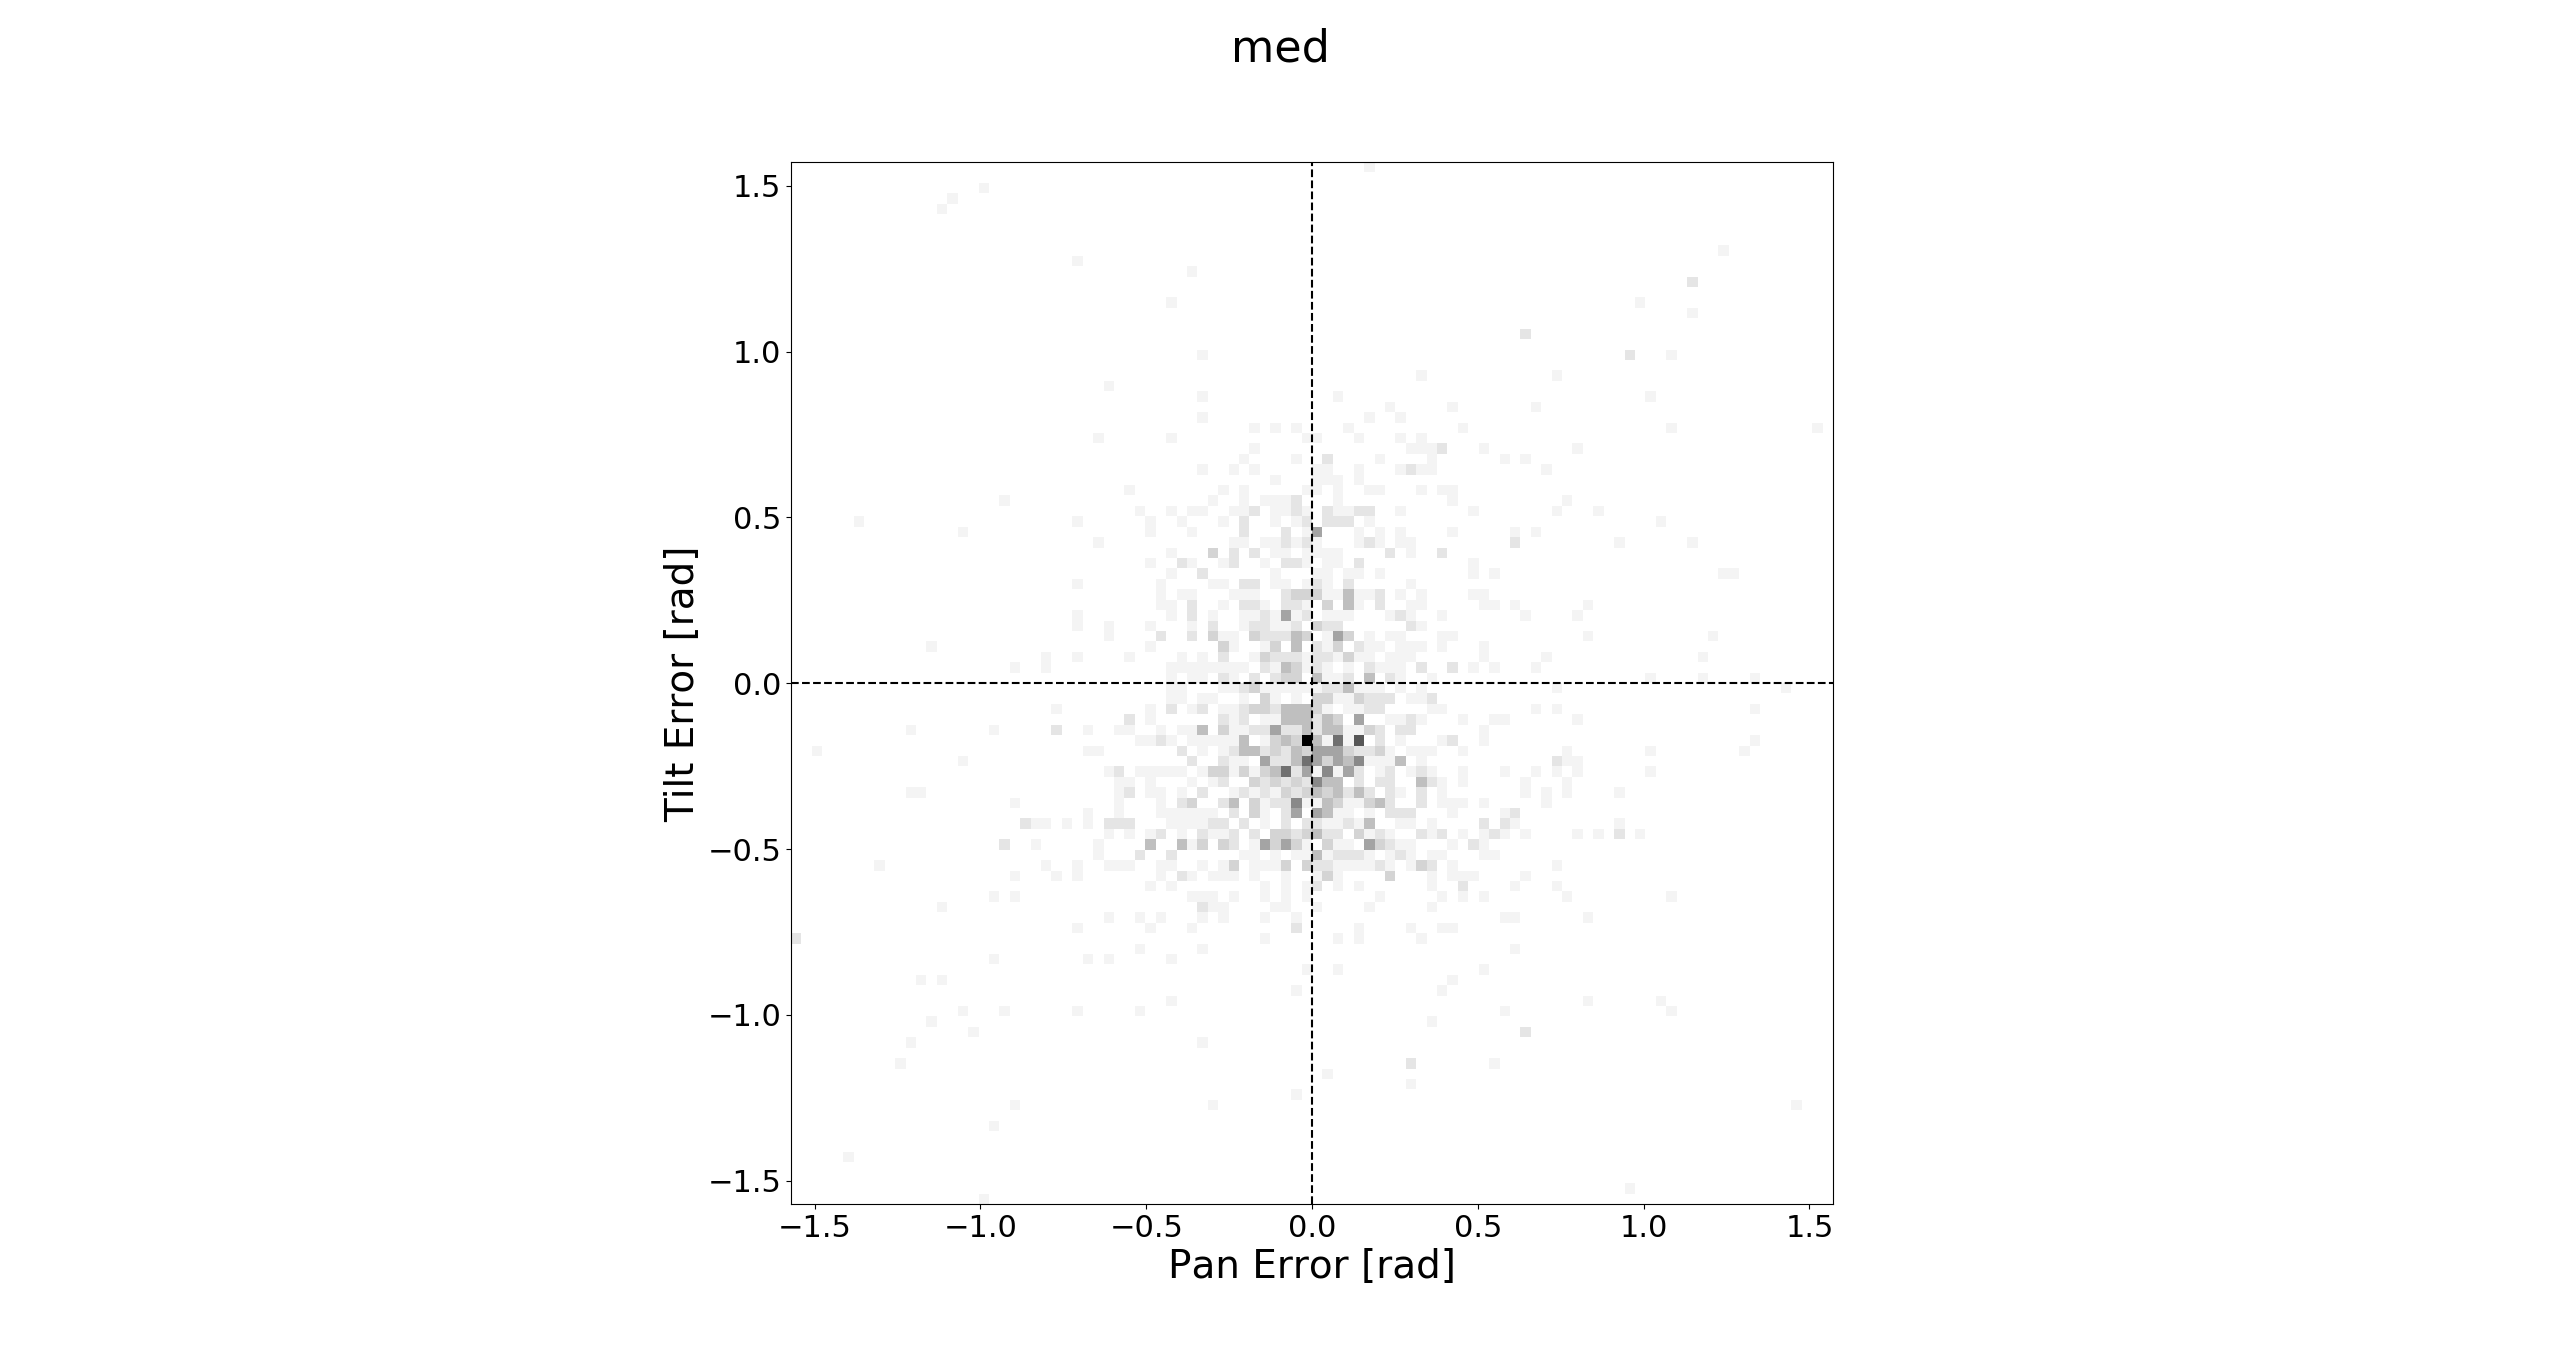
\includegraphics[clip, trim=450 0 450 110, width=0.8\columnwidth]{figures/err_med.png}}

  %\subfloat[Results for the $m_h$ setting.]{\label{fig:err-results-hi}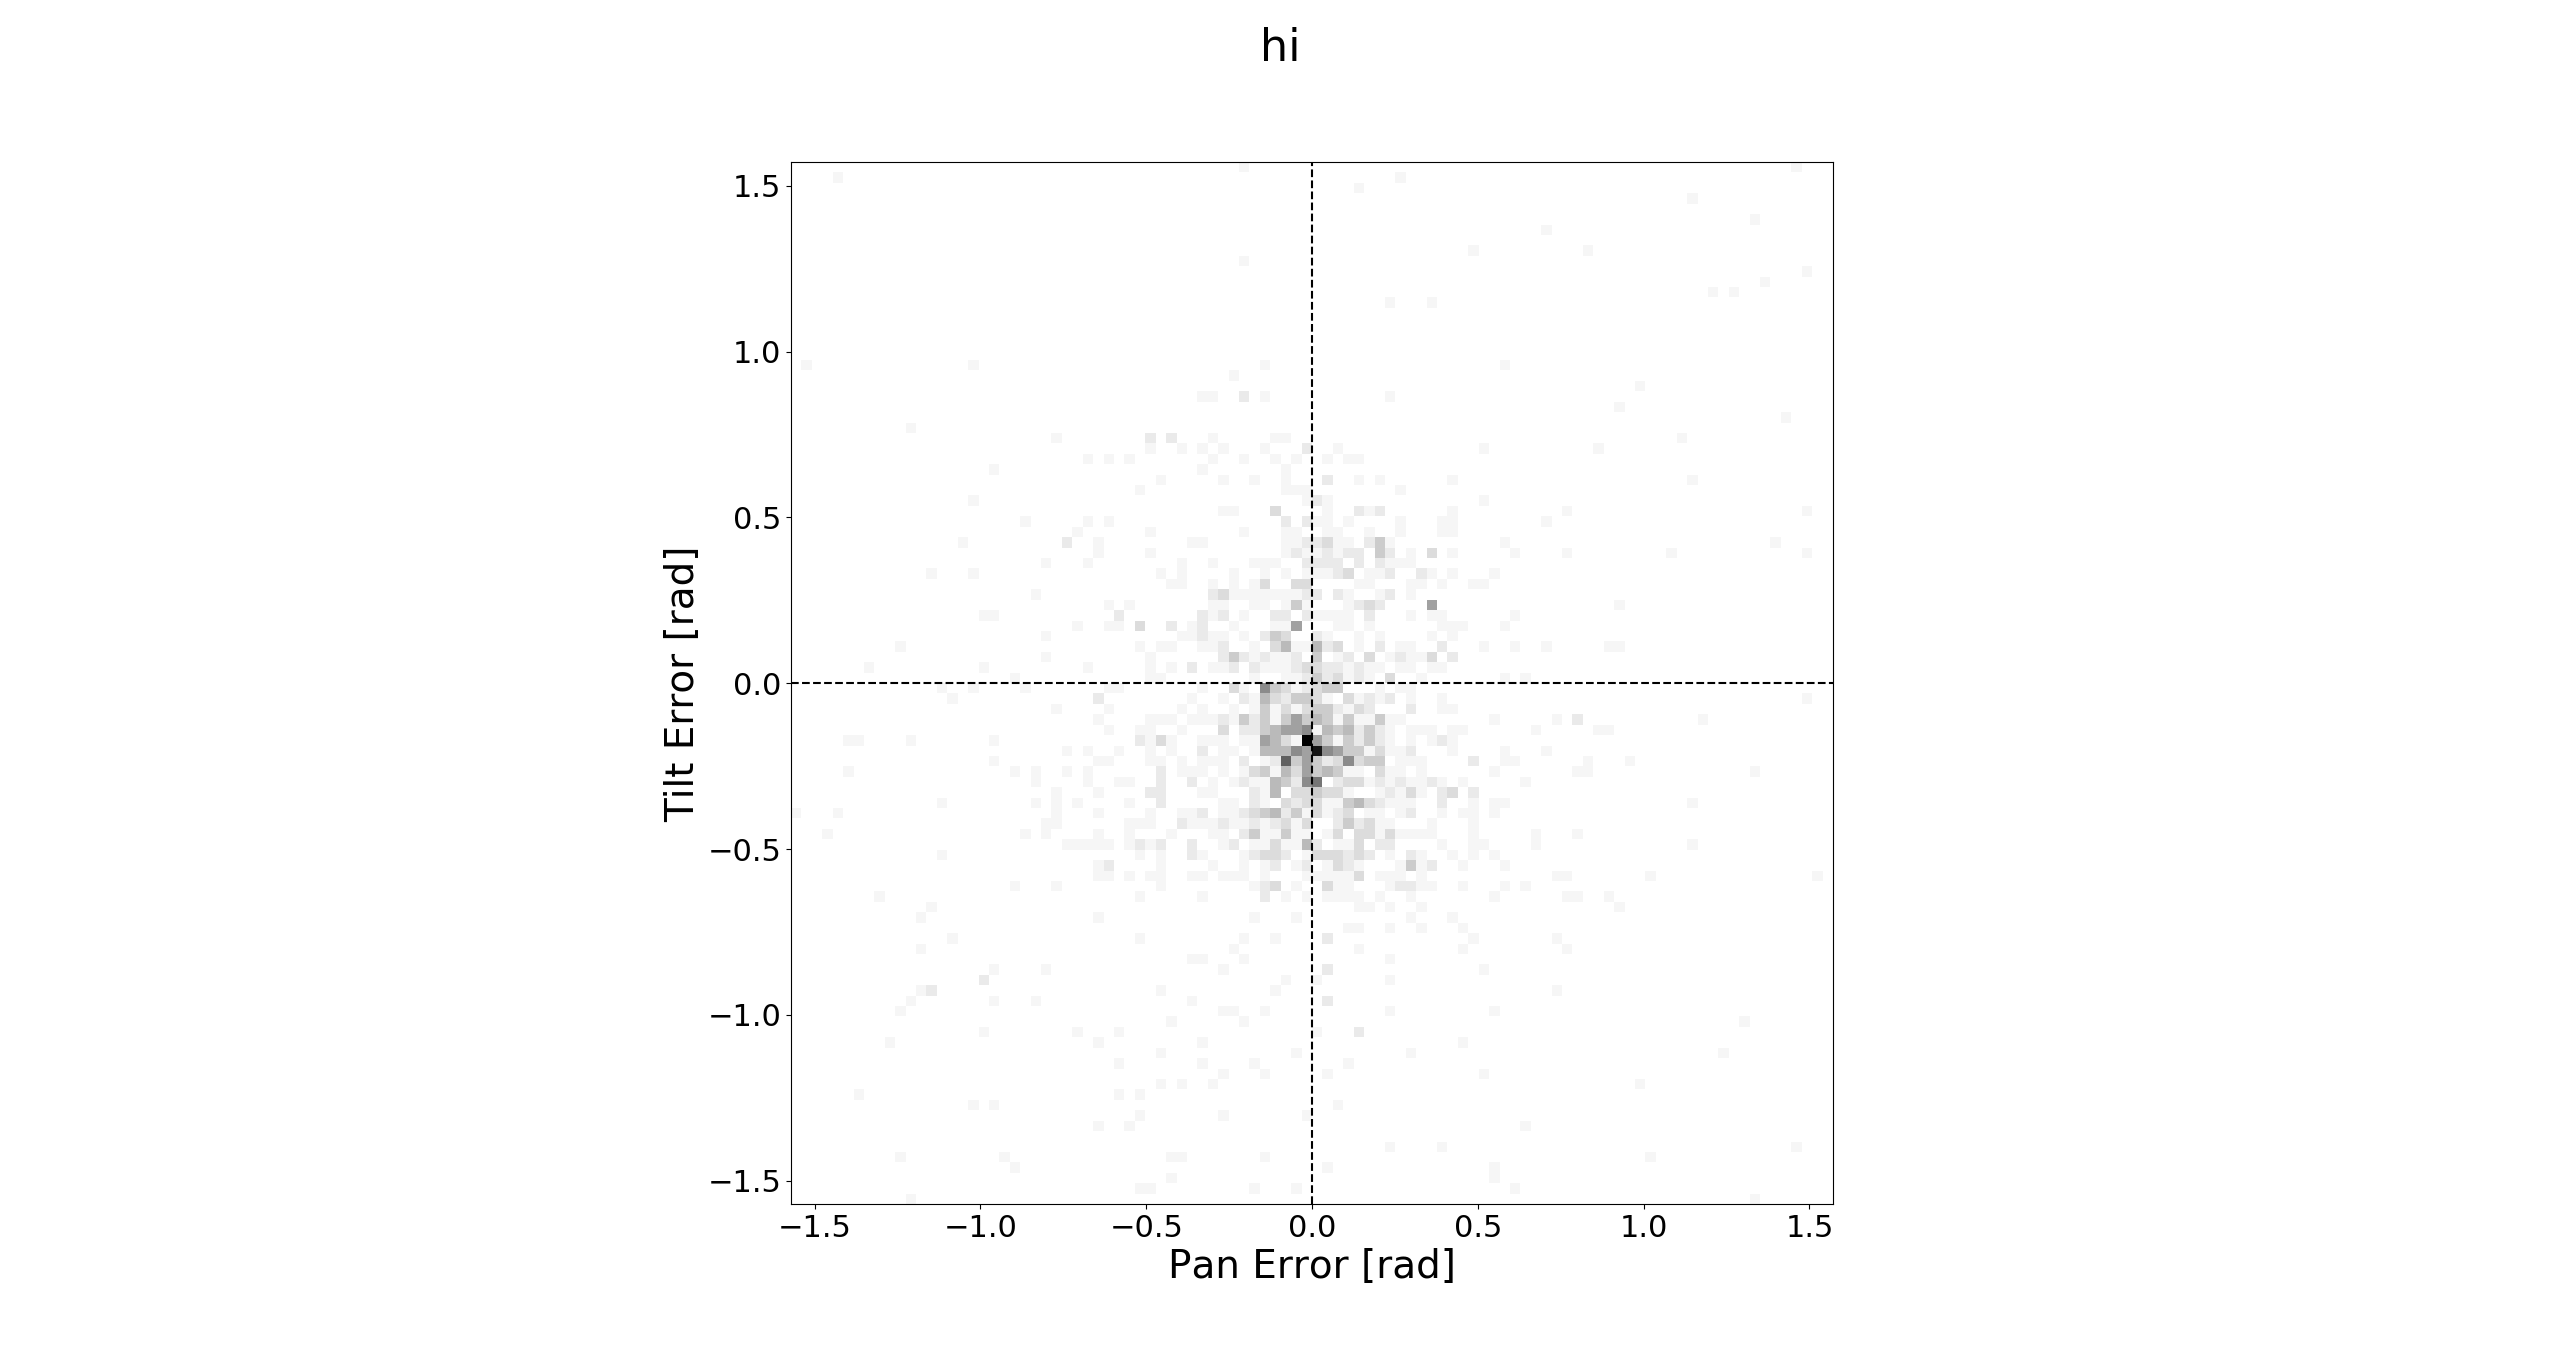
\includegraphics[clip, trim=450 0 450 110, width=0.8\columnwidth]{figures/err_hi.png}}

  %\caption{Angular error data for the 3 gradient settings. }\label{fig:err-results}
%\end{figure}

%\begin{figure}
  %\centering
  %\subfloat[The medians. ]{\label{fig:err-boxplot-median}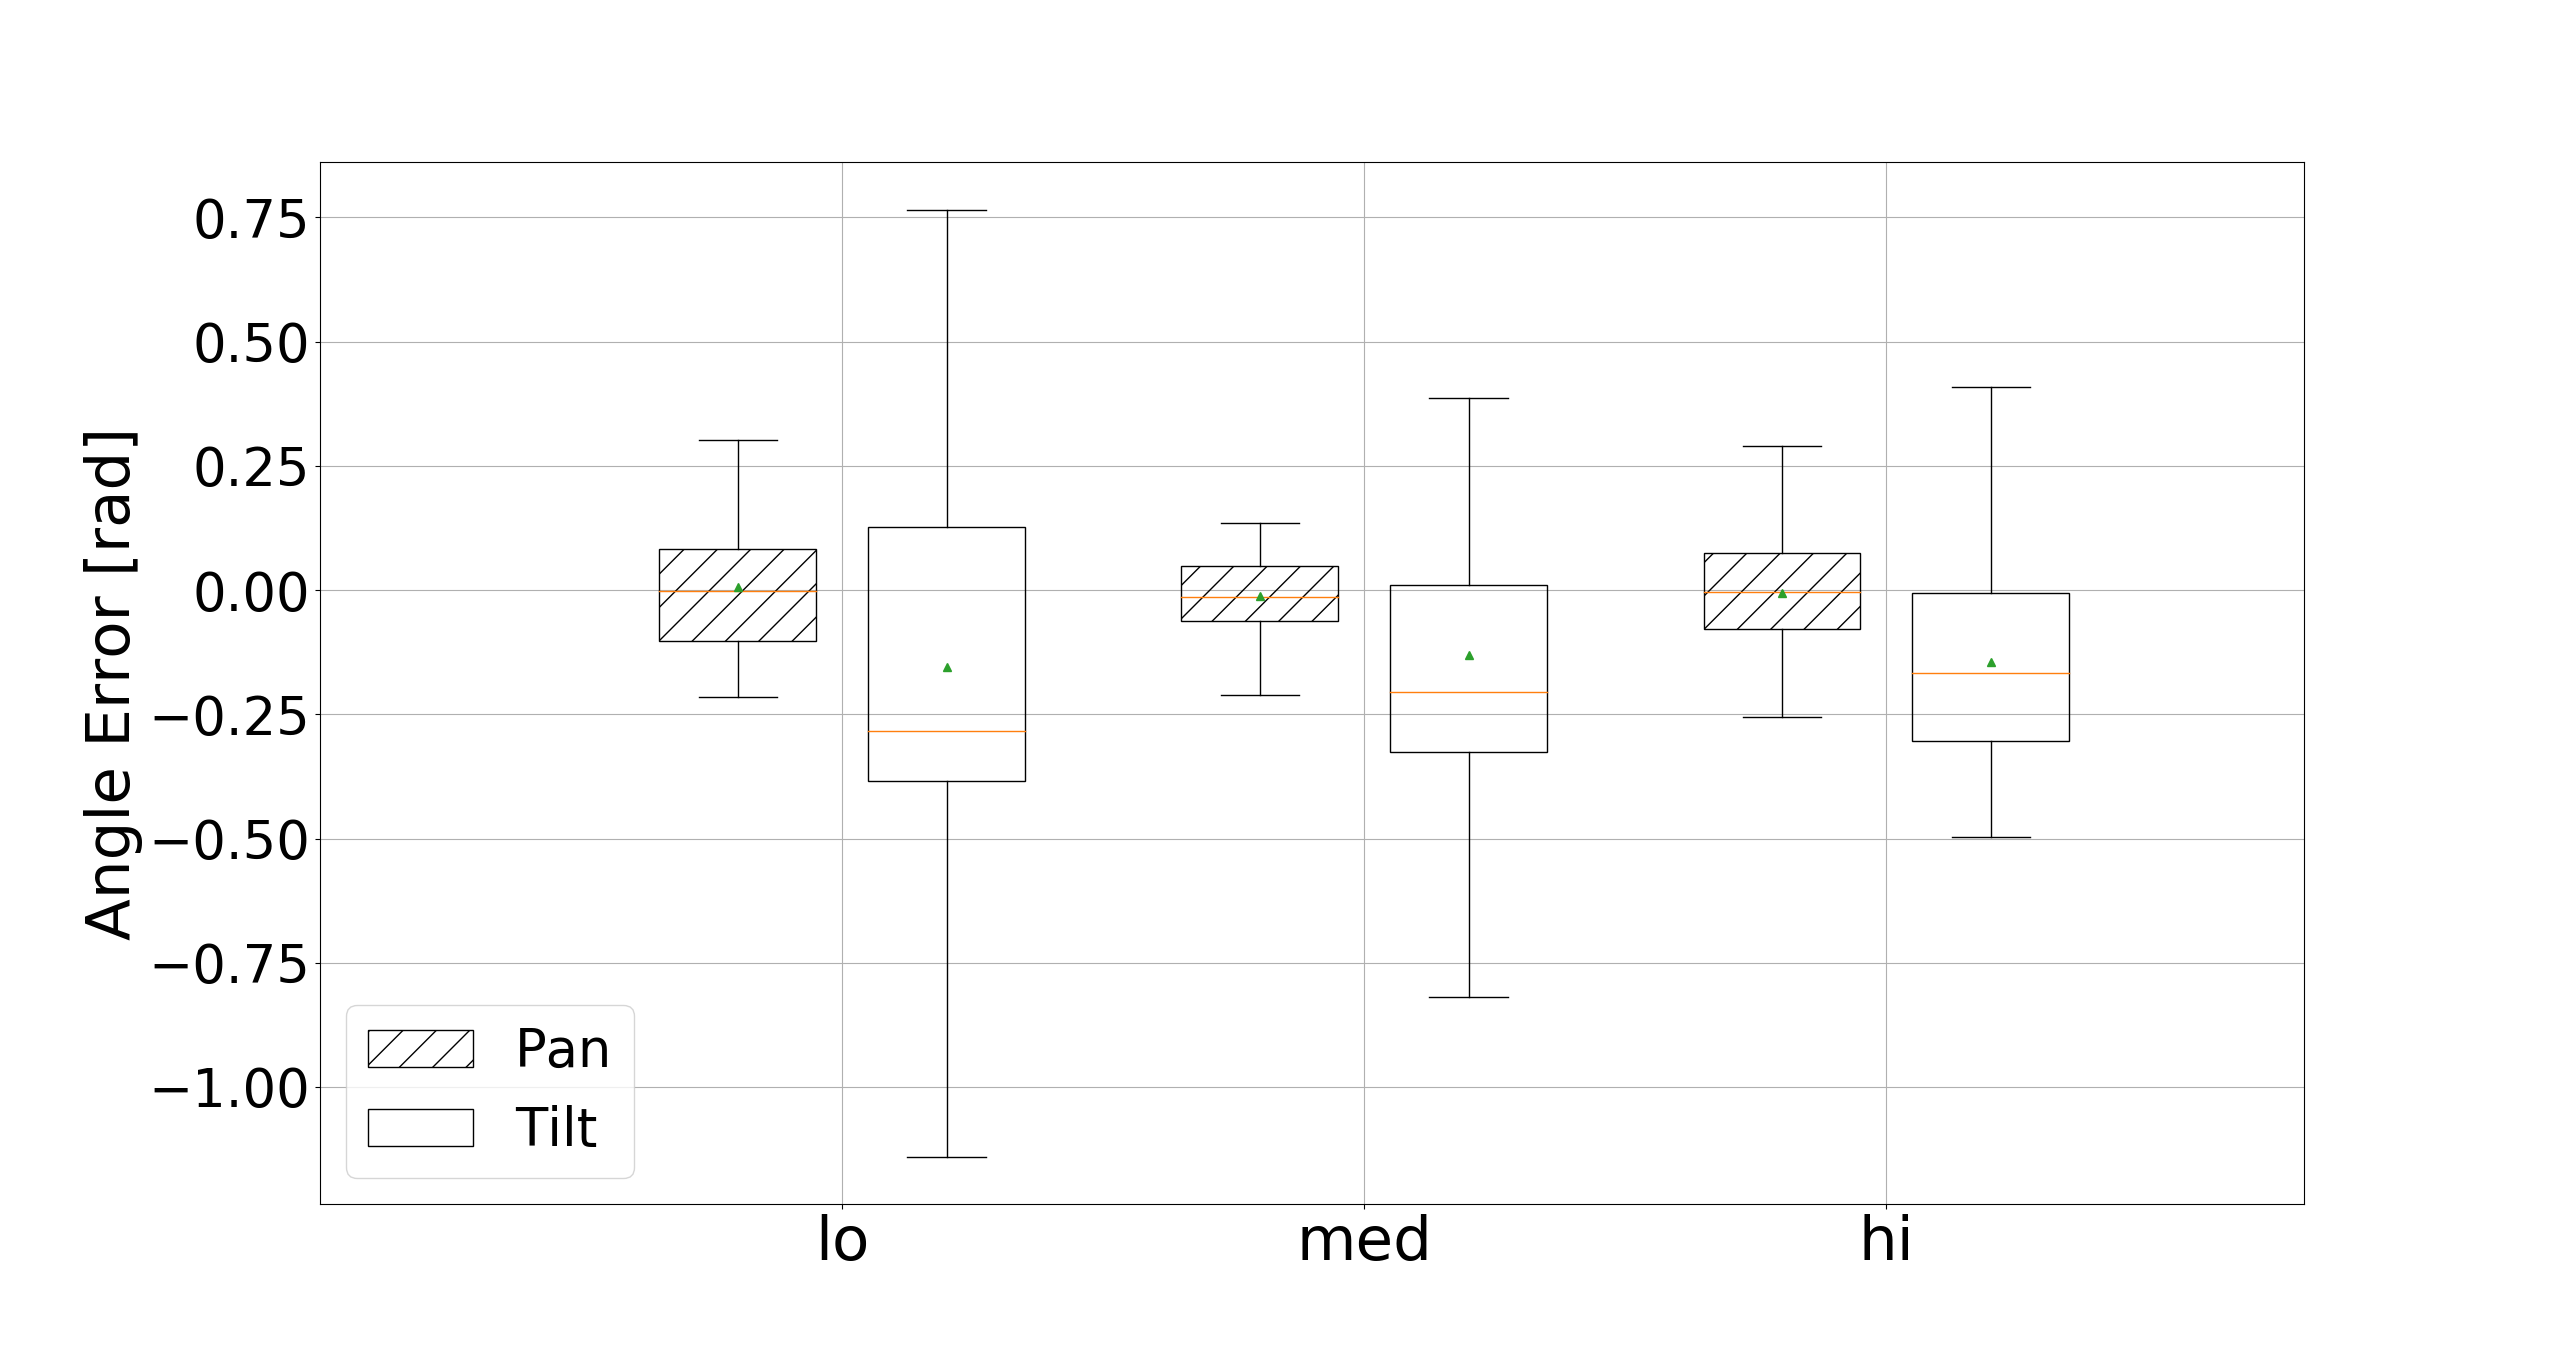
\includegraphics[clip, trim=20 -70 100 100, width=1.0\columnwidth]{figures/err_boxplot_medians.png}}

  %\subfloat[The standard deviations. ]{\label{fig:err-boxplot-std}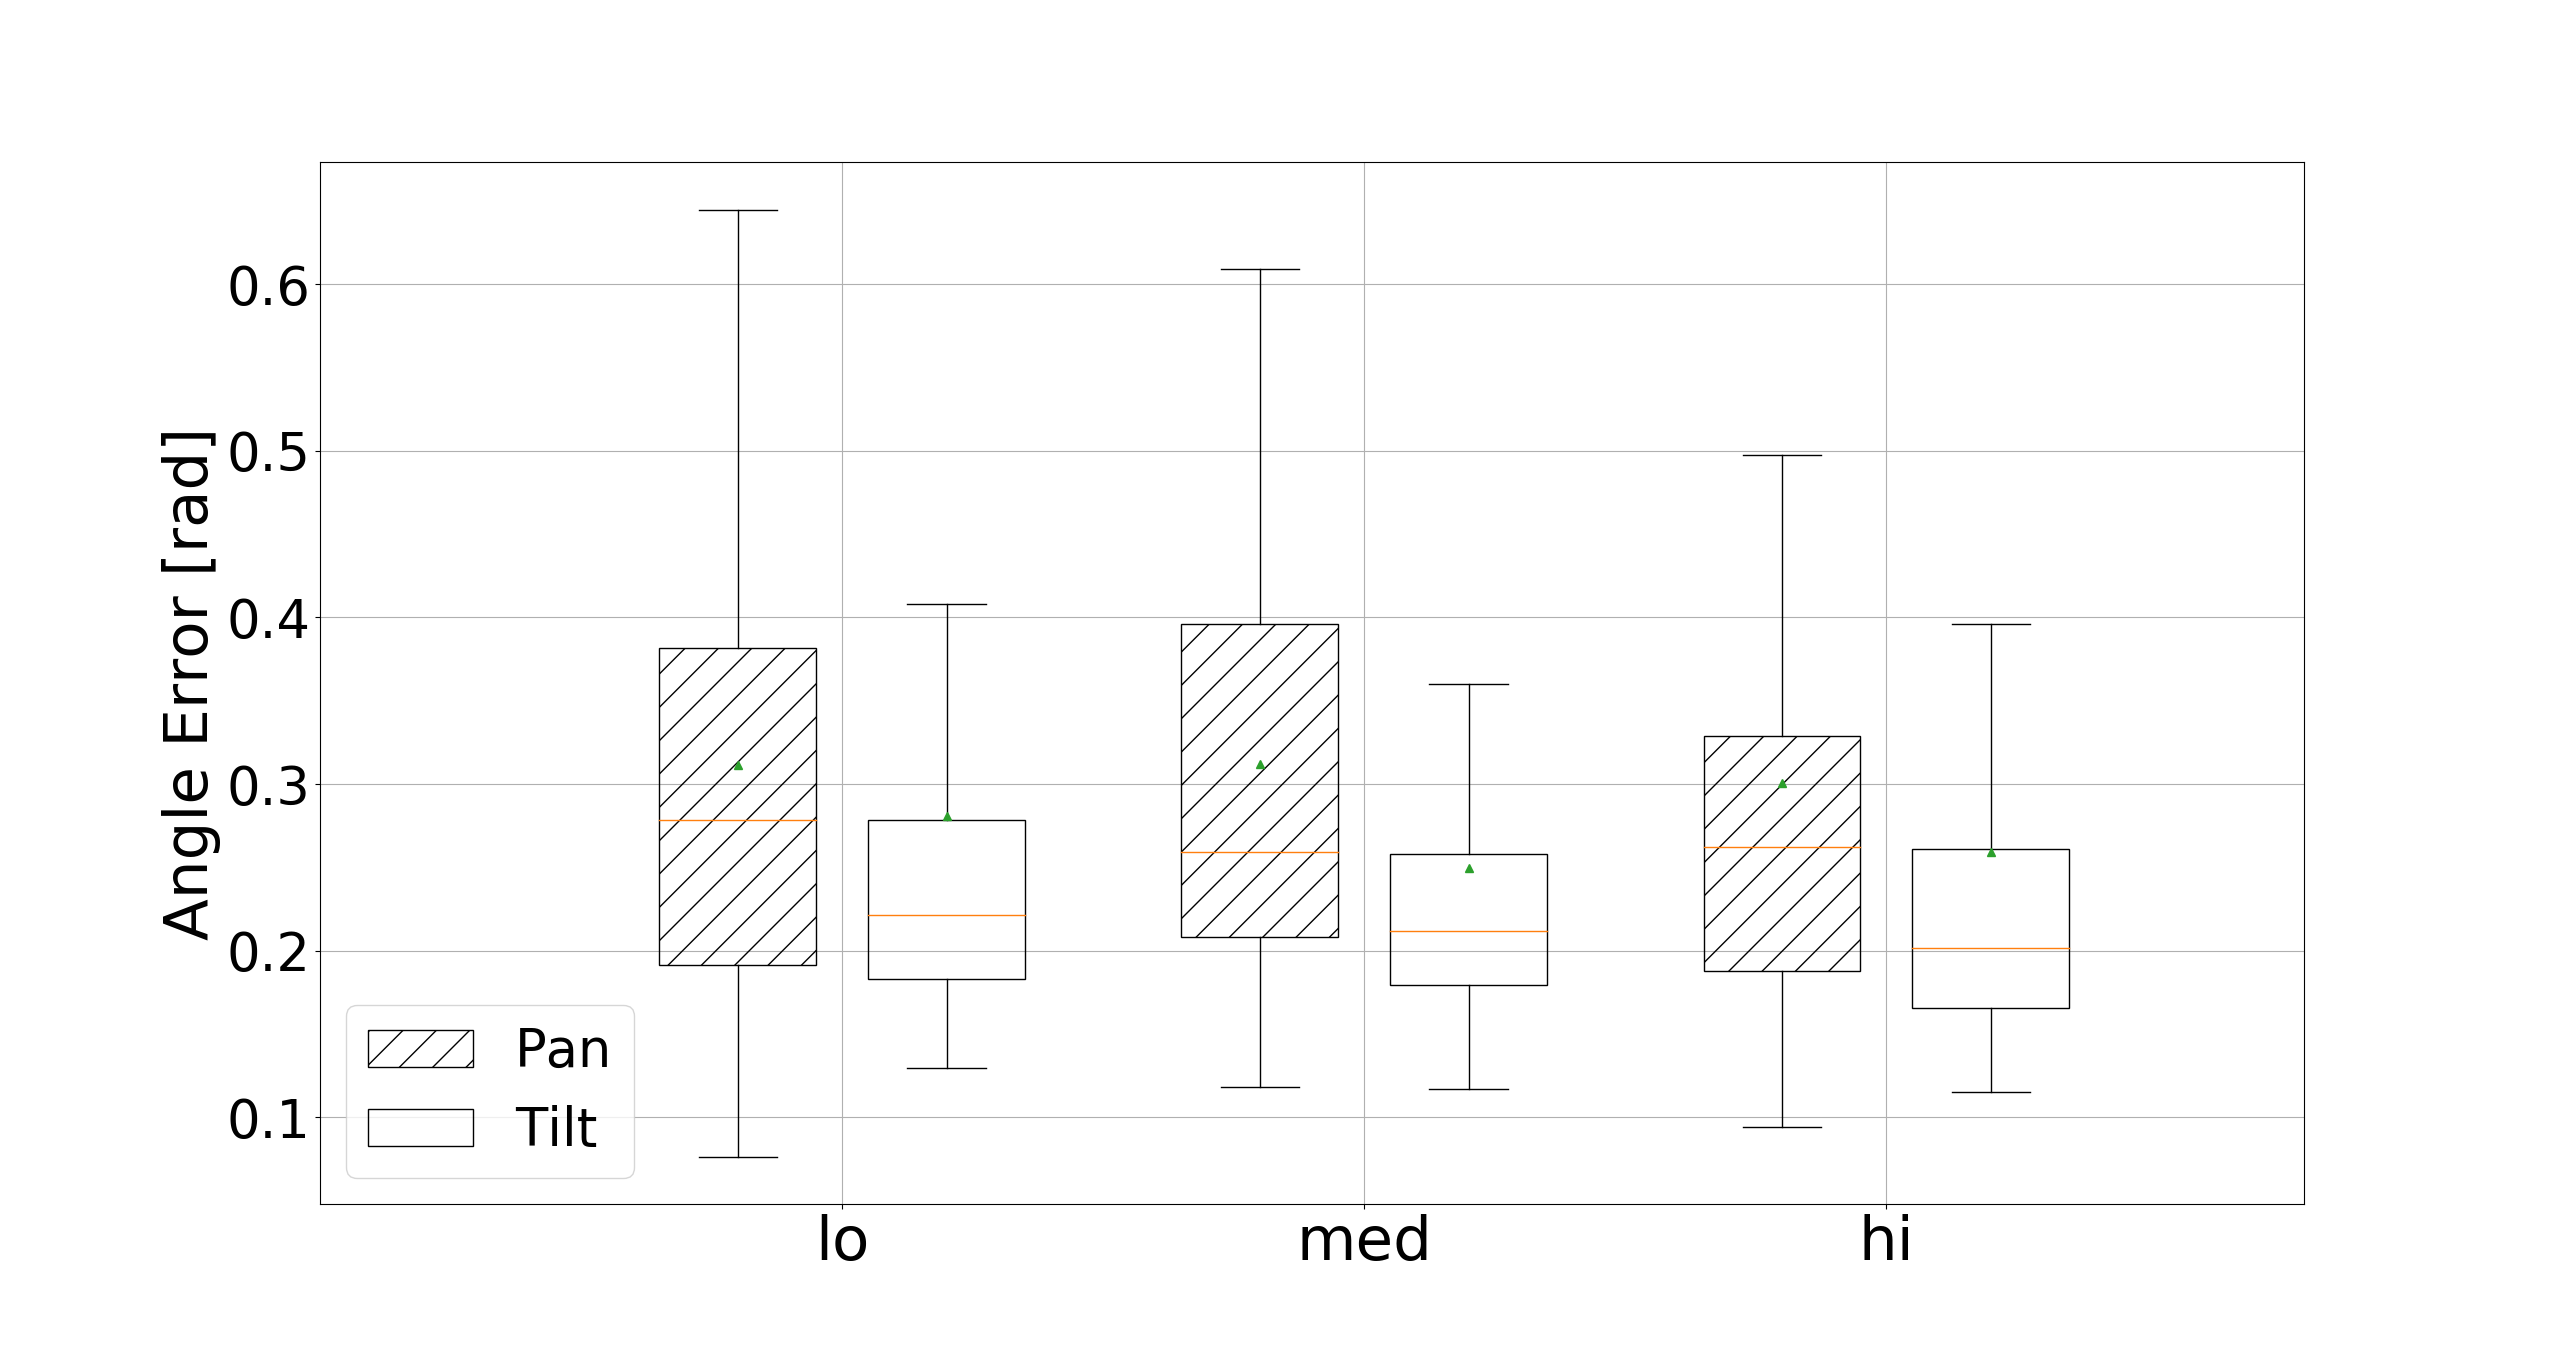
\includegraphics[clip, trim=20 -70 100 100, width=1.0\columnwidth]{figures/err_boxplot_std.png}}

  %\caption{Boxplots for the error medians and standard deviations. }\label{fig:err-boxplot}
%\end{figure}

%\begin{table}
  %\centering
  %\caption{A table of the pan and tilt angular error results collected from $G1$. The results include the absolute average error ($\mu_{abs}$), average error ($\mu$) and standard deviations ($\sigma$) given in radians, as well as the Spearman ($R$) correlation scores.}\label{tab:results}
  %\begin{tabular}{llcccc}
    %\toprule
    %\multicolumn{2}{c}{} & $\mu_{abs}$ & $\mu$ & $\sigma$ & $R$ \\\midrule
	 %& $m_l$ & 0.23 & -0.02 & 0.32 & 0.75 \\%\cmidrule{2-6}
    %Pan  & $m_m$ & 0.21 & -0.01 & 0.28 & 0.77 \\%\cmidrule{2-6}
	 %& $m_h$ & 0.22 & -0.05 & 0.31 & 0.75 \\\midrule
	 %& $m_l$ & 0.40 & -0.14 & 0.46 & 0.38 \\%\cmidrule{2-6}
    %Tilt & $m_m$ & 0.32 & -0.12 & 0.36 & 0.48 \\%\cmidrule{2-6}
	 %& $m_h$ & 0.34 & -0.16 & 0.39 & 0.55 \\
    %\bottomrule
  %\end{tabular}
%\end{table}

%\begin{table}
  %\centering
  %\caption{A table summarising the target search results of the participants in $G2$ (P1 - P3). The results include the average error ($\mu$) and standard deviation ($\sigma$), given in radians in the pan and tilt dimensions.}\label{tab:vi-results}
  %\begin{tabular}{llcccccc}
    %\toprule
    %\multicolumn{2}{c}{} & \multicolumn{2}{c}{$m_l$} & \multicolumn{2}{c}{$m_m$} & \multicolumn{2}{c}{$m_h$} \\
    %\multicolumn{2}{c}{} & $\mu_l$ & $\sigma_l$ & $\mu_m$ & $\sigma_m$ & $\mu_h$ & $\sigma_h$ \\\midrule
	 %& P1 &  0.25 & 0.44 &  0.21 & 0.45 &  0.29 & 0.40 \\% \cline{2-8}
    %Pan  & P2 &  0.18 & 0.85 &  0.05 & 0.49 & -0.08 & 0.32 \\% \cline{2-8}
	 %& P3 & -0.10 & 0.67 & -0.08 & 0.61 & -0.08 & 0.50 \\ \midrule
	 %& P1 & -0.17 & 0.21 & -0.10 & 0.2  & -0.25 & 0.21 \\% \cline{2-8}
    %Tilt & P2 & -0.87 & 0.26 & -0.05 & 0.21 & -0.15 & 0.18 \\% \cline{2-8}
	 %& P3 & -0.57 & 0.31 & -0.57 & 0.45 & -0.38 & 0.39 \\% \hline
    %\bottomrule
  %\end{tabular}
%\end{table}

%\subsection{Pan Results}

%\cref{fig:err-results} and the median and mean points from the boxplots in \cref{fig:err-boxplot} show that the data in the pan dimension are approximately normally distributed around zero.
%However, a Shapiro-Wilkes test score below the critical threshold do not give enough confidence to consider the data as normally distributed and we therefore analyse the data through non-parametric techniques. 

%For the data collected from $G1$, there is a strong linear correlation between the participants' guesses and the targets' true pan angles, shown by the high Spearman correlation scores of approximately 0.75 ($p < 0.01$) for all of the datasets, with the $m_m$ setting displaying the marginally best result of 0.77.
%The 3 settings have similar average errors and standard deviations, with the $m_m$ setting again producing the marginally best results with the smallest average error and standard deviation.
%However, the differences are relatively small (approximately 6\%) and are not significant enough (Friedman test $p = 0.92$) to conclude that the pitch gradient has an effect on the target acquisition accuracy performance in the pan dimension. 

%The data collected from $G2$ follow a similar trend to $G1$: the error in the pan dimension is centred around \SI{0}{\radian} with similar standard deviations across all 3 settings.
%Unfortunately, not enough samples could be collected to draw any final conclusions.
%However, these results are in line with results from previous work~\cite{zwiers2001spatial}, indicating that the groups with partial and normal eyesight respond with similar levels of accuracy to spatialised sound when presented with simple tasks. 

%These results show that both groups managed to find the targets with reasonable level of accuracy and that the pan error is robust to variations in the pitch's rate of change; a useful result in support of the effectiveness of this audio interface.

%\subsection{Tilt Results}\label{sec:tilt-results}

%The data within the tilt dimension were also found to be non-normal following scores below the critical threshold from the Shapiro-Wilkes test.
%The Spearman test for the data reveals a reasonably significant correlation between the participants' guesses and the actual locations of the targets, with correlation scores of approximately 0.38 for $m_l$, 0.48 for $m_m$ and the $m_h$ gradient giving the strongest correlation score with 0.55 ($p < 0.01$ for all 3 settings).
%This indicates that the participants generally interpret the cues from the varying the pitch correctly and are mostly successful at pointing the camera in the correct tilt angle.

%The average errors of the datasets are relatively close to one another, with the $m_l$ setting producing the largest absolute error and standard deviation at \SI{0.40}{\radian} and \SI{0.46}{\radian} respectively.
%The $m_m$ and $m_h$ settings have similar absolute errors of \SI{0.32}{\radian} and \SI{0.34}{\radian} respectively.
%This is in line with the correlation scores, with $m_l$ giving the worst result and $m_h$ giving the best results overall, with highest correlation score and relatively low absolute angular errors and standard deviation, marginally beating $m_m$. 

%Since the data are not normally spread and there is significant levels of noise within the data which may contaminate the mean values, we use the medians to analyse the datasets.
%For this, the Friedman test is used on the participants' error medians and it was found that there is a significant difference between the 3 settings' datasets ($p < 0.01$).
%A post-hoc analysis with a Wilcoxon signed rank test and a critical threshold with a Bonferroni correction applied ($\alpha=0.016=\frac{0.05}{3}$) shows that both the $m_m$ and $m_h$ settings are significantly different from the $m_l$ setting ($p=0.0014<\alpha$ for both settings), but that the $m_m$ and $m_h$ settings do not produce significantly different results from one another ($p=0.42>\alpha$).
%This indicates there is an inflection point where increasing $m$ produces diminishing returns and that we cannot conclude that the $m_h$ setting is better than the $m_m$ gradient.
%However, both settings conclusively produce more accurate results than the $m_l$ setting.

%From \cref{fig:err-boxplot-median} it can be seen that the median data show a significant skewing to the negative side, indicating a potential bias amongst the experiment's participant-base that must be taken into account.
%From the results, it is not completely clear what causes this negative bias in the pitch dimension.
%However, a possible explanation is that the floor introduces a position constraint within a user's mind, since the target cannot appear below the ground.
%It can potentially appear above the user's head though, giving variable upper an lower limits that depend on the user's height and individual perception.
%Future improvements to our audio interface should consider a non-linear increase in pitch as a function of tilt angle instead of the linear one we used in this work to remedy this bias.

%The results collected from $G1$ and $G2$ show that a varying pitch tone can convey the tilt angle of a target to a human using bone-conducting headphones with accuracy levels similar to that in literature~\cite{bujacz2011sonification,katz2011spatial,zotkin2004rendering}.
%They also highlight a clear and significant difference between the 3 different pitch gain gradients, with the $m_l$ setting giving the lowest acquisition accuracy, while $m_m$ and $m_h$ give similar accuracy levels closest to the target's true tilt. 

%\subsection{Participants with Visual Impairment's Feedback}

%After the experiments with the participants with visual impairments in $G2$ were completed, we took the opportunity to collect their feedback on the audio interface's current implementation and gather suggestions for improvements for future iterations.
%When asked about their opinions on current assistive systems available on the market, the general consensus was that these systems are typically prohibitively expensive, too complex and cumbersome to be useful for everyday use.
%Indeed, they seemed quite enthusiastic about a guidance system that they can use on a mobile phone.

%They were generally satisfied with the guidance interface in its current form and had little problem learning how to use it.
%However, they, along with the participants in $G1$, reported auditory fatigue caused by long-term exposure to the sinusoidal audio tone.
%We were aware of this issue before the experiments were conducted and have considered replacing the simple sine wave tone with more natural and pleasant sounds.
%For example, musical instruments can be used to play different notes and scales to indicate different elevation angles~\cite{brewster1998using}.
%Furthermore, they suggested adding some voice component or tone prompt to confirm when they are on target, inform them of other important events or happenings or simply to intermittently assure them that the system is still active.
%The former two suggestions were intentionally ignored in order to purely evaluate how accurately the audio tone can guide a user to the target.
%Going forward, however, these suggestions will be helpful for a potential commercial release version of the guidance system to make the guidance instructions clearer and to intermittently reassure users that they are still on the right course, for example.

%On the hardware, only one participant had reservations regarding the choice of bone-conducting headphones, citing cost concerns. 
%However, he indicated that he could justify purchasing a set of bone-conducting headphones if he were to use them throughout the day to avoid cutting off environmental sounds.
%None of the participants had any technical issues using the headphones or mobile device and were able to properly use and interpret the guidance instructions.

%\section{Conclusion and Future Work}\label{sec:conclusion}

%In this work, we present an audio-based guidance interface that uses a spatialised audio tone with varying pitch to direct a user with visual impairments to point a camera toward a target. 
%We also present and discuss a set of experiments that were conducted to determine the interface's effectiveness and performance, as well as some subjective feedback that was collected from legally blind participants. 

%Using a set of bone-conducting headphones, we found that a spatialised audio tone with a varying pitch can successfully convey the pan and tilt angles of a target.
%The angular errors made by the participants are in line with those from previous research using similar audio guidance instructions.
%We also found that varying the pitch's rate of change influences the accuracy of the system in the tilt dimension without affecting the performance in the pan dimension.
%The steeper, $m_h$ and $m_m$ pitch gradients were found to produce the best accuracy results in general.

%Feedback from the participants with visual impairments was mostly positive and they agreed with the choice of bone-conduction headphones that do not inhibit normal hearing.
%However, they noted that the sine wave audio signal induced audio fatigue after extended exposure, something noted by the other participants as well, and suggested that more full-bodied, natural sounds be used instead.
%Using vocal feedback in conjunction with the current audio signal was also suggested. 

%These results are more interesting from a design point of view than an end-user's. 
%Indeed, we have shown that this audio guidance interface is effective at directing an average person, but more data are needed with the intended audience in order to decisively conclude that this interface will be effective in an indoor guidance system for people with vision impairments. 
%Nevertheless, these data are a good indication of what to expect when we evaluate this audio interface with a greater number of people with limited vision.
%Once we have determined that the intended audience can effectively use this type of guidance instruction, we can start adding more user-oriented features (e.g.\ voice prompts, more pleasant tones, etc.) and integrate them into our guidance system prototype. 

\bibliographystyle{splncs04}
\bibliography{bib}

\end{document}
